
\documentclass{article}

\usepackage{jragonfyre}
\theoremstyle{remark}
\newtheorem*{question}{Question}
\newtheorem*{fact}{Fact}
\newtheorem{exercise}{Exercise}

\newcommand\diam{\operatorname{diam}}

\title{Bergelson Notes 7/4}
\author{Jason Schuchardt}

\begin{document}

\maketitle

\section{Questions}

Question: What is isomorphism, why are
$2x\mod{1}$, the tent map, and the logistic
map isomorphic?

\begin{definition}
    If $f:X\to X$ then for all $x_0\in X$,
    the \emph{semiorbit} of $x_0$ is
    \[ \set{f^n(x_0): n\ge 0} \text{ (note $f^0(x_0)=x_0$)}. \]

    Why semiorbit? Because if $f$ is invertible, then we 
    can also talk about the \emph{orbit}
    \[ \set{f^n(x_0): n\in\ZZ}.\]
\end{definition}

Sometimes we want to think about set valued functions, and 
talk about fixed points in this context. We won't do it 
now, but they're important in economics and game theory.
However, you should feel that they are lurking in the
background, since they show up naturally when 
we take preimages. See Figure \ref{fig:preimages}

\begin{figure}
    \centering
    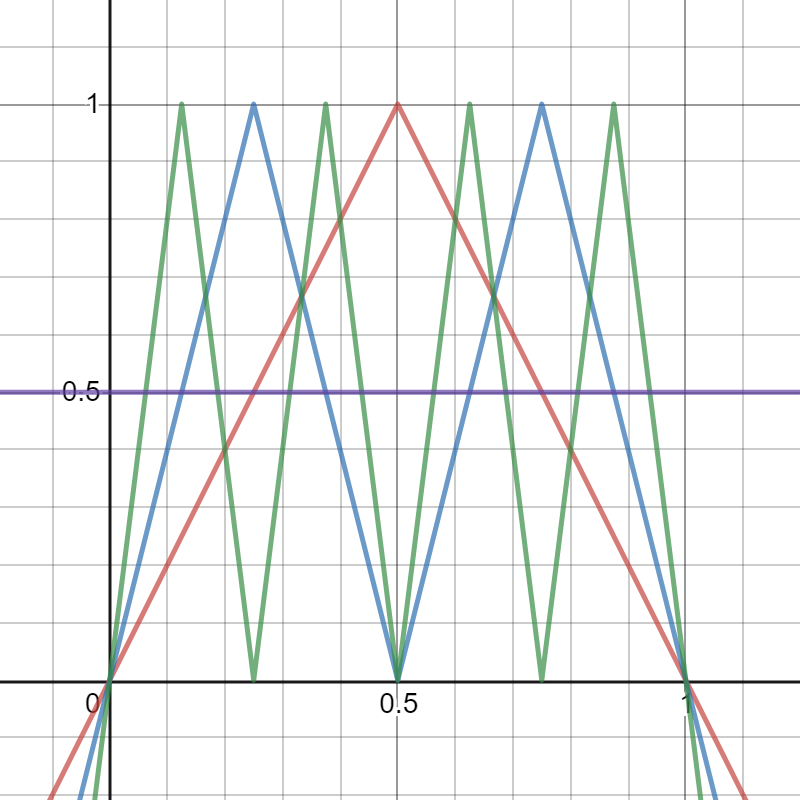
\includegraphics[width=0.6\textwidth]{tent-preimage.png}
    \caption{Iterates of the tent map, and the line $y=1/2$}
    \label{fig:preimages}
\end{figure}

\begin{question}
Sensitive dependence on initial conditions 
should be for invertible 
functions? It's false for noninvertible functions. 
See Figure \ref{fig:preimages}.
We are talking about the condition
\[ f^n(x) - f^n(y) > \epsilon \]
\end{question}

Exercise still remains for the map of
\[\bmat 2 & 1 \\ 1 & 1 \emat \]
on $\TT^2$.
Why is it invertible?

Suppose we write 
\[\bmat 2 + \epsilon_1 & 1 + \epsilon_2 \\
1+\epsilon_3 & 1 + \epsilon_4 \emat \]
this is still a mapping mod $1$.

Seminar: Work more on $\TT^2$.
Stress that $\TT^n = \RR^n/\ZZ^n$, so 
\[ \TT=\RR/\ZZ = \set{\text{the set of cosets, $\ZZ+t$} : t\in[0,1] }
\]

Another example would be $X=\set{0,1}^\ZZ$, $f:X\to X$ is shift,
if $x$ is a sequence, the shift  $\sigma x$ is
\[ (\sigma x)_n= x_{n+1}. \]

\begin{question}
Last time you mentioned topological entropy.
Maybe we can talk about it.
\end{question}

\begin{definition}
    Let $(X,d)$ be a compact metric space,
    $T:X\to X$ is called \emph{topologically
    mixing} if for all open nonempty $U$, $V$
    $\subseteq X$, there is some $n$ such that
    \[ T^nU\cap V \ne \nullset. \]
\end{definition}

This is like in physics, we have laminar and turbulent flow.
Periodic points are ``laminar-like,'' points with dense orbit
are ``turbulent-like.'' Chaotic systems have both types
together.

\begin{question}
Start with a function $f(x)=x$.
Can you perturb by an arbitrarily small amount to make it chaotic? 

By an arbitrarily small amount, we mean that for any
$\epsilon$, we can add a function $g$
with \[ \sup_{x\in[0,1]} |g(x)|<\epsilon. \]
\end{question}

\begin{exercise}
    Given $X=[0,1]$, equipped with Lesbesgue measure, $\mu$, a
    transformation $T:[0,1]\to[0,1]$ is called 
    \emph{mixing} if for any measurable $A,B \subseteq [0,1]$,
    $\mu(A), \mu(B) > 0$, 
    then 
    \[ \mu(A\cap T^{-n}B) \to \mu(A)\mu(B) \]
    as $n\to \infty$.

    Assume that for all measureable $A\subseteq [0,1]$,
    $\mu(T\inv A)=\mu(A)$. I.e., that $T$ is 
    \emph{measure preserving}.
\end{exercise}

Why is this a good definition?
\[ \mu(A\cap B) = \mu(A)\mu(B) \]
is the definition of the independence of sets $A$ and $B$.
Consider the sets in Figure \ref{fig:independence},
they are independent, and this is a typical picture 
of what independence looks like in practice.
The sets somehow come from different coordinates.
\begin{figure}
    \centering
    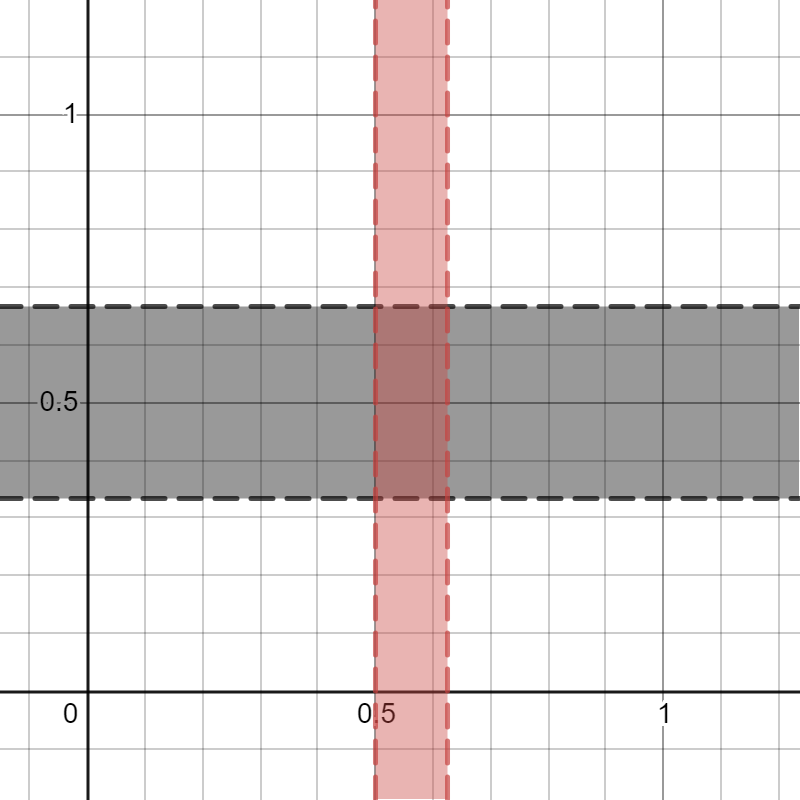
\includegraphics[width=0.6\textwidth]{independence.png}
    \caption{Two independent sets in $[0,1]\times [0,1]$.}
    \label{fig:independence}
\end{figure}

\begin{exercise}
    (i) Find a sequence, $(A_n)$, of pairwise independent sets in 
    $[0,1]$.
    (ii) Find a sequence $(A_n)\subseteq [0,1]$ of 
    \emph{mutually independent sets}. This means that for
    any $k$, and for all $A_{n_1},A_{n_2},\ldots,A_{n_k}$,
    with the indices distinct,
    \[\mu(A_{n_1}\cap A_{n_1}\cap \cdots \cap A_{n_k})
    = \mu(A_{n_1})\mu(A_{n_2})\cdots \mu(A_{n_k}).
    \]
\end{exercise}

What is an example of three mutually independent sets?
Consider the space $[0,1]^3$. Take the sets $A\times [0,1]^2$,
$[0,1]\times B \times [0,1]$, $[0,1]^2\times C$,
where $A,B,C$ are positive measure subsets of $[0,1]$.

Another way to think about mixing in terms of independence
is that sets tend to become independent as we iterate $T\inv$.

\begin{question}
    Why did we take $T\inv$ in the definition of mixing?
\end{question}

\begin{example}
    This example should show why we want $T\inv$.

    Consider the tent map, $2x\mod{1}$, the map 
    \[\bmat 2 & 1 \\ 1 & 1 \emat :\TT^2\to\TT^2,\]
    and the logistic map.

    Is it clear that the first three preserve Lebesgue measure?

    The first two have slope two, so the image has twice the 
    area, but the preimage of an interval consists of two 
    intervals, each with half the area.

    \begin{exercise}
        In order to establish that $T$ is measure-preserving
        (for Lebesgue measure),
        it is enough to check that it holds for intervals.

        The reason is that it suffices to check that
        the measure-preserving property holds for a 
        generating set for the $\sigma$-algebra.
    \end{exercise}

    Thus preimage preserves measure, but the direct image
    shrinks measure, so it's not as good for us.

    In general, mathematics prefers working with preimages. 
    This is true in
    topology as well. We define $f$ to be 
    continuous to be that $f\inv(U)$ is open for all open 
    $U$ in the codomain.
\end{example}

There is a famous example, that we can't tell in this class,
because it involves mixing cocktails. Instead the story will
be about milkshakes.

You take milk and chocolate syrup, and start shaking it.
Shaking is a measure preserving transformation, since 
liquids are incompressible. If the quality of the shaking is good,
then it will be mixing, and you will get a good cocktail\dots, 
milkshake.

Note: $\sigma$-additive and countably additive will have the 
same meaning for us.

Seminar: Please give the general definition of measure,
as a $\sigma$-additive function.

Consider topologically mixing transformation $T$,
we can consider 
\[U\cap T^{-n}V \overset{?}{=} T^{-n}(T^nU\cap V)
\overset{?}{\ne} \nullset,\]
and the claim is that it doesn't matter whether we have 
$n$ or $-n$ in the definition for topologically mixing, since 
we don't want to measure the size.

\begin{exercise}
    If you have a matrix $A$ acting on $\RR^n$, then $A$ 
    is measure preserving (for the Lebesgue measure)
    if and only if $|\det(A)|=1$.
\end{exercise}

Can we generalize this? If we have a general differentiable map,
how can we determine if it is measure preserving? 
Sketch: At each point, we can take the best linear approximation
to the function, the Jacobian matrix. The determinant of the 
Jacobian should measure how much the function changes Lebesgue 
measure locally. 

\section{Isomorphism}

\begin{definition}
    Let $X_1$, $X_2$ be spaces. If they are topological spaces,
    then 
    \[ X_1\cong X_2 \]
    if $X_1$ and $X_2$ are homeomorphic.

    Now assume (for convenience) that $X_1$, $X_2$ are compact
    metric spaces, and $f_i : X_i\to X_i$ are continuous 
    maps. Then the systems, $(X_1,f_1)$ and $(X_2,f_2)$ are 
    isomorphic as topological dynamical systems if 
    there exists a homeomorphism $\phi : X_1\to X_2$ such that
    the diagram
    \[
        \begin{tikzcd}
        X_1 \arrow[d, "f_1"] \arrow[r, "\phi"] & X_2 \arrow[d, "f_2"] \\
        X_1 \arrow[r, "\phi"]                  & X_2                 
        \end{tikzcd}   
    \]
    commutes.
\end{definition}

\begin{example}
    We can easily give an example of things that are not
    isomorphic. The easiest way is to select nonhomeomorphic
    spaces, like $[0,1]$ and $\set{0,1}^\NN$.

    Another reasonable question is:
    Given two rotations of the circle, $r_\alpha: x\mapsto x+\alpha$,
    $r_\beta:x\mapsto x+\beta$. When are they isomorphic?
    Suppose that $\alpha$ and $\beta$ are irrational.
    Otherwise, if $\alpha,\beta$ are rational, it is easy,
    to see rotation by $180$ and $90$ degrees are different.
\end{example}

\begin{exercise}
    (i) Given two irrational rotations of the circle, $r_\alpha$,
    $r_\beta$. When are they isomorphic? 
    They are not in general.
    (ii) Similarly, if we take matrices 
    \[\bmat 1 & 1 \\ 1 & 0 \emat, \quad 
    \bmat 2 & 1 \\ 1 & 1 \emat, \quad
    \bmat 5 & 1 \\ 19 & 4 \emat \]
    when are they isomorphic as maps $\TT^2\to \TT^2$.

    The answer might depend on a computable invariant of the
    system.
\end{exercise}

We have four examples:
\begin{enumerate}
    \item $2x\mod{1}$,
    \item the tent map,
    \item $S^1\to S^2$, $z\mapsto z^2$,
    \item $\set{0,1}^\NN\toby{\sigma}\set{0,1}^\NN$, the shifting
        map. $(\sigma x)_n = x_{n+1}$.
\end{enumerate}

They should all be isomorphic.
However, they are not isomorphic in our topological sense.
The first map is not even continuous. 
$S^1$ and $[0,1]$ are different topological spaces,
since removing one point from $(0,1)$ disconnects the space,
but removing any point from $S^1$ still leaves a connected space.
Finally the last topological space is homeomorphic to the 
Cantor set, and therefore by considering connectedness, it 
cannot be the same as $S^1$ or $[0,1]$.

The correct notion of isomorphism for our purposes will 
be measure theoretic, and should have the same general shape.

We now want $\phi:X_1\to X_2$ to be an isomorphism of measure
spaces.
How would we define this? 
\begin{definition}
    $\phi:(X_1,\mu_1)\to (X_2,\mu_2)$
    is an isomorphism of measure spaces if 
    it is a measure preserving
    almost everywhere bijection. I.e.,
    $\phi$ is defined on a subset of $X_1$ 
    of full measure and has values on 
    some set of full measure, and 
    we have $\phi^*\mu_2=\mu_1$, meaning 
    that for all measurable subsets $B$ of $X_2$,
    \[ \mu_2(B) = \mu_1(\phi\inv(B)). \]

    More precisely again,
    $(X_i,\mu_i)$ are measure spaces, $\mu_i(X_i)=1$.
    Then $X_1$ is isomorphic to $X_2$ if there exist sets
    $\widetilde{X_i}\subset X_i$, with $\mu_i(\widetilde{X_i})=1$,
    \newcommand\wtil\widetilde
    and there is $\phi:\wtil{X_1}\to\wtil{X_2}$ such that
    for all $A\subseteq X_2$ (or $\wtil{X_2}$), such that
    \[ \mu_1(\phi\inv(A)) = \mu_2(A).\]

    The next step to rigorizing this is to allow $\phi$ to 
    represent a class of maps defined up to measure zero.
\end{definition}

\begin{exercise}
With this definition, $[0,1]$ and $\set{0,1}^\NN$ are isomorphic
as measure spaces, indeed as dynamical systems.
\end{exercise}

\begin{exercise}
    $[0,1]^2$ and $[0,1]$ are also measure theoretically
    isomorphic. We suddenly lose a notion of dimension when
    we move to measure theoretic dynamics.
\end{exercise}

This is good for dynamics, since we no longer worry about 
peculiarities of spaces, but instead the peculiarities 
of dynamics.

Is $L^2[0,1]$ a space of functions? It's a space of equivalence
classes of functions. This is different. We can't evaluate any 
element of $L^2[0,1]$ at any point, since we can always change
the function on any set of measure $0$.

\begin{exercise}
Can you give me an example of a Hilbert space that is a 
functional space, which is made
not of classes of equivalence functions, but of actual functions.
The answer is yes.
\end{exercise}

Seminar: Touch on Hilbert and Banach spaces.

\section{Banach Fixed Point Applications}

Examples of applications of the Banach fixed point theorem.

\subsection{Finding roots}

Let $F:[a,b]\to \RR$, and assume that $F$ is continuous,
$F(a) < 0$, $F(b) > 0$. We know that a root exists, but how 
can we find it? Assume also that $F'(x)$ exists, and 
\[ 0 < c_1 \le F'(x) \le c_2. \]

Let 
\[ f(x) = x-\lambda F(x)\quad  (\lambda\ne 0) \tag{*}\label{eqn:star}. \]
We are looking for $x$ such that
$f(x) = x$, in which case $F(x)=0$. Now differentiating
\eqref{eqn:star}, we get
\[ f'(x) = 1- \lambda F'(x),\]
so 
\[ 1-\lambda c_2 \le f'(x) \le 1 -\lambda c_1. \]
Now choose $\lambda$ so that $|f'(x)| \le c < 1$
for all $x\in [a,b]$.

Then Banach fixed point theorem gives us a fixed point, which
is a zero of our original function.

The derivative condition follows from the mean value theorem
We want \[\abs{f(x)-f(y)} < c\abs{x-y},\]
this follows from $f(x)-f(y) = f'(\theta_{xy}) (x-y)$ for 
some $\theta_{xy} \in (x,y)$ together with the uniform
bound on the derivative.


\subsection{Solving linear equations}

We have a transformation $T:\RR^n\to\RR^n$ such that 
$Tx = Ax+b$, with $x,b\in\RR^n$, $A\in M_{n\times n}(\RR)$.
We want solutions to $Tx=x$.

What does it mean for our matrix to be a contraction? It 
depends on the metric on $\RR^n$. We will go through three 
important cases.

We want to find conditions under which $T$ is a contraction.
The three cases to consider are $d_1$, $d_2$, $d_\infty$.

\begin{enumerate}
    \item[$d_\infty$:] The condition is 
        \[\sum_{j=1}^n a_{ij} \le c < 1\]
        for all $i=1,\ldots,n$.
    \item[$d_1$:] The condition is 
        \[ \sum_{i=1}^n a_{ij} \le c < 1 \]
        for all $j=1,\ldots,n$.
    \item[$d_2$:] The condition is 
        \[ \sum_{i,j} a_{ij}^2 \le c < 1. \]
\end{enumerate}


In $\RR^n$ we can introduce norm $\|x\|_2$
by 
\[ \sqrt{\sum_i x_i^2}=d_2(x,0).\]
Then $d_2(x,y) = \norm{x,y}$.

Question: Is the general condition that we take $p$-norm of rows,
$q$-norm of these $p$-norms.

\begin{exercise}
    Give the answer for $d_p$, for general $p\in [1,\infty]$.
\end{exercise}

Question: For Euclidean norm, is there a way to express it 
in terms of traces and eigenvalues?
 
This is still $n^2$ operations, so do we have sufficient conditions
that are easier to check?

\begin{exercise}
    If $\abs{a_{ij}} < \frac{1}{n}$ for all $i,j$, then
    all three conditions are satisfied.

    If $a_{ij} > \frac{1}{n}$ for all $i,j$, then none of the 
    three conditions are satisfied.
\end{exercise}

\subsection{Solving differential equations}

What is this thing:
\[ \frac{dy}{dx} = f(x,y), \quad y(x_0)=y_0? \]
It is an ordinary differential equation, since 
we only have one variable.
How do we know a solution exists?

The general result wasn't obtained for a while. Special cases
were known by some people. The first one was Picard. He 
established solution in a neighborhood of $(x_0,y_0)$.

\begin{exercise}
    Look up these people: Picard, Brouwer, Sperner, Lebesgue,
    Peano, Lipschitz.
\end{exercise}

If you want a general solution, the best theorem is by Peano.
Peano is famous for Peano axioms, a space filling curve,
and his theorem on the existence of global solutions to 
ODEs.

Convenient assumption is that 
\[ f(x,y_1)-f(x,y_2) \le M |y_1-y_2| \]
for all $(x,y_i)$ in some domain $G$ around $x_0,y_0$.
This condition is called a Lipschitz condition on $y$.

\begin{theorem}[Picard]
There exists $d>0$ such that on the interval
\[ |x-x_0|\le d \]
our equation has a unique solution
$y=\phi(x)$.
\end{theorem}

\begin{proof}[Proof sketch]
    \begin{enumerate}
        \item Move to an equivalent integral equation,
            \[ \phi(x) = y_0 \int_{x_0}^x f(t,\phi(t))\,dt \]
        \item Now we need to choose $t$.
            Since $f$ is continuous in $G$, and $G$ is compact
            there exists $K$ such that 
            \[|f(x,y)| \le K\]
            for all $x,y\in G$.
            Then choose $d$ so that (i) if $|x-x_0| < \delta$,
            then $|y-y_0| < Kd$, and (ii) $Md < 1$.
        \item Then $Md$ will be the constant for the Banach
            fixed point theorem.
        \item We are moving to a subspace to make everything work.
    \end{enumerate}
\end{proof}

Question: Is the convex body exercise still true for star 
shaped sets? 

Answer: Yes. 

Note taker's comment: I think you'll want star shaped about 
every point in an open neighborhood.

\end{document}